
%-----------------------------------------------------
\chapter[Giao thoa ánh sáng và điều kiện xảy ra giao thoa ánh sáng]{Giao thoa ánh sáng \\và điều kiện xảy ra giao thoa ánh sáng}
\section{Lý thuyết}
\subsection{Hiện tượng nhiễu xạ ánh sáng}
Hiện tượng truyền sai lệch so với sự truyền thẳng khi ánh sáng gặp vật cản gọi là hiện tượng nhiễu xạ ánh sáng.

Hiện tượng nhiễu xạ chỉ có thể giải thích được nếu thừa nhận ánh sáng có tính chất sóng. Mỗi ánh sáng đơn sắc coi như một sóng có bước sóng xác định.
\begin{center}
	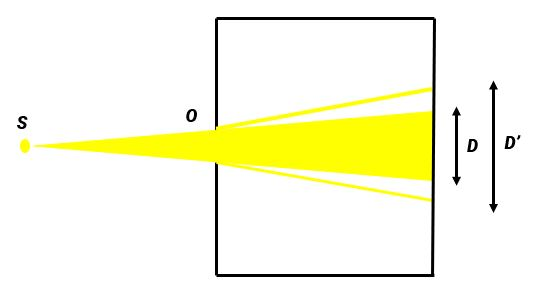
\includegraphics[scale=0.7]{../figs/VN12-PH-33-L-020-1-2.JPG}
\end{center}

\subsection{Hiện tượng giao thoa ánh sáng}
\begin{description}
	\item[Hiện tượng giao thoa ánh sáng] là hiện tượng hai chùm ánh sáng kết hợp khi chồng lên nhau sẽ tạo ra những chỗ chúng tăng cường lẫn nhau, và những chỗ chúng triệt tiêu lẫn nhau tạo ra những vân sáng, vân tối xen kẽ nhau. 
	
	Hiện tượng giao thoa ánh sáng là một bằng chứng thực nghiệm quan trọng khẳng định ánh sáng có tính chất sóng.
	\item[Hai nguồn sáng kết hợp] là hai nguồn sáng  phát ra hai sóng ánh sáng có cùng bước sóng và hiệu số pha dao động giữa hai nguồn không thay đổi theo thời gian.
	\item[Điều kiện xảy ra giao thoa ánh sáng] là hai chùm sáng giao nhau phải là hai chùm sáng kết hợp.
\end{description}



\subsection{Vị trí các vân}
Ta ký hiệu: 
\begin{itemize}
	\item $a$ là khoảng cách giữa hai nguồn kết hợp,
	\item $D$ là khoảng cách từ hai nguồn đến màn,
	\item $\lambda$ là bước sóng ánh sáng,
	\item $x$ là tọa độ của điểm đang xét trên màn.
\end{itemize}
\begin{center}
	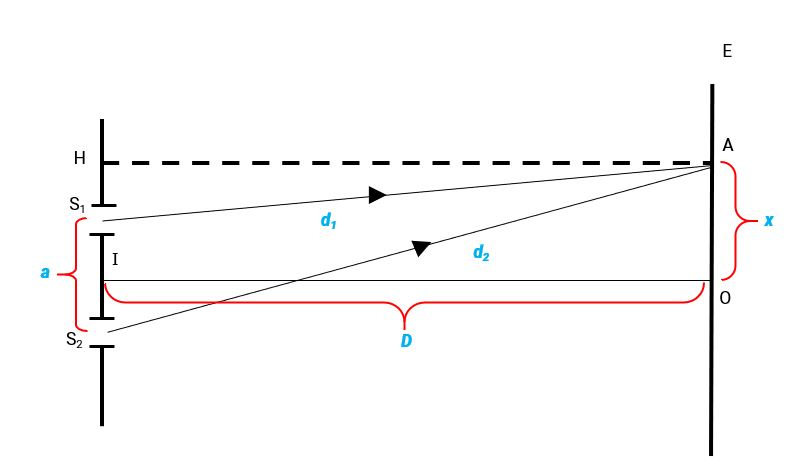
\includegraphics[scale=0.7]{../figs/VN12-PH-33-L-020-1-1.JPG}
\end{center}

\subsubsection{Hiệu quang lộ và vân giao thoa}
Hiệu đường đi $\delta$ trong trường hợp $a\ll D$:
\begin{equation}
	\delta = d_2-d_1=\dfrac{ax}{D}.  
\end{equation}
Tính chất vân tại A phụ thuộc hiệu quang lộ:
\begin{itemize}
	\item Để tại A là vân sáng thì: $$d_2-d_1=k\lambda$$ với $k=0; \pm 1; \pm 2,...$
	\item Để tại A là vân tối: $$d_2-d_1=\left(k+\dfrac{1}{2}\right) \lambda$$ với $k= \pm 1; \pm 2,...$
\end{itemize}
\subsubsection{Vị trí vân sáng và vân tối}
Vị trí vân sáng:
\begin{equation}
	x=k\dfrac{\lambda D}{a},\ k=\pm 1; \pm 2,...
\end{equation}

Vị trí vân tối: 
\begin{equation}
	x=\left(k'+\dfrac{1}{2}\right) \dfrac{\lambda D}{a},\ k'=0; \pm 1; \pm 2,... 
\end{equation}


\subsubsection{Khoảng vân}
Khoảng vân $i$ là khoảng cách giữa hai vân sáng, hoặc hai vân tối liên tiếp.

Công thức tính khoảng vân: 
\begin{equation}\label{eq:khoangvan}	
	i=\dfrac{\lambda D}{a}.	
\end{equation}

Tại O là vân sáng bậc 0 của mọi bức xạ chính là vân chính giữa hay vân trung tâm.

\subsubsection {Ứng dụng đo bước sóng ánh sáng}
Trong thí nghiệm giao thoa với khe Young, bằng cách đo $i$, $a$, $D$, bước sóng ánh sáng $\lambda$ được suy ra từ công thức \eqref{eq:khoangvan}.
\section{Bài tập tự luyện}
\begin{enumerate}[label=\bfseries Câu \arabic*:]
	
	%========================================
	\item \mkstar{1} [5]
	\cauhoi
	{Trong thí nghiệm Y-âng, tại vị trí vân tối thì
		\begin{mcq}(1)
			\item Độ lệch pha của hai sóng từ hai nguồn kết hợp thỏa mãn $\delta \varphi = (2k+1) \dfrac{\pi}{2}$ với $k \in Z$. 
			\item Hai sóng đến từ hai nguồn kết hợp vuông pha với nhau. 
			\item Hiệu quang trình từ hai nguồn kết hợp thỏa mãn $d_{2} - d_{1} = (2k+1)\dfrac{\lambda}{2}$ với $k \in Z$. 
			\item Hiệu quang trình từ hai nguồn kết hợp thỏa mãn $d_{2} - d_{1} = (2k+1)\lambda$ với $k \in Z$.  
		\end{mcq}
	}
	
	\loigiai
	{		\textbf{Đáp án:  C.}
		
		Trong thí nghiệm Y-âng, tại vị trí vân tối thì hiệu quang trình từ hai nguồn kết hợp thỏa mãn $d_{2} - d_{1} = (2k+1)\dfrac{\lambda}{2}$ với $k \in Z$. 
		
	}
	
	%========================================
	\item \mkstar{1} [5]
	\cauhoi
	{Hiện tượng giao thoa chứng tỏ rằng 
		\begin{mcq}(2)
			\item ánh sáng là sóng ngang. 
			\item ánh sáng là sóng điện từ. 
			\item ánh sáng có bản chất sóng. 
			\item ánh sáng có thể bị tán sắc. 
		\end{mcq}
	}
	
	\loigiai
	{		\textbf{Đáp án: C.}
		
		Hiện tượng giao thoa chứng tỏ rằng ánh sáng có bản chất sóng.
		
	}
	
	%========================================
	\item \mkstar{1} [5]
	\cauhoi
	{Hiện tượng giao thoa ánh sáng chỉ quan sát được khi hai nguồn ánh sáng là hai nguồn 
		\begin{mcq}(2)
			\item cùng màu sắc. 
			\item đơn sắc. 
			\item cùng cường độ. 
			\item kết hợp. 
		\end{mcq}
	}
	
	\loigiai
	{		\textbf{Đáp án: D.}
		
		Hiện tượng giao thoa ánh sáng chỉ quan sát được khi hai nguồn ánh sáng là hai nguồn kết hợp.
		
	}
	
	%========================================
	\item \mkstar{1} [13]
	\cauhoi
	{Trong thí nghiệm Y-âng về giao thoa ánh sáng, với k là số nguyên. Công thức dùng để xác định vị trí vân sáng trên màn quan sát là
		\begin{mcq}(2)
			\item $x = \dfrac{a}{D} k \lambda$. 
			\item $x = \dfrac{D}{2a} \lambda$. 
			\item $x= k \dfrac{\lambda D}{a}$. 
			\item $x = \dfrac{D}{a} (k+0,5) \lambda$. 
		\end{mcq}
	}
	
	\loigiai
	{		\textbf{Đáp án: C.}
		
		Công thức xác định vị trí vân sáng trong giao thoa khe Y-âng là $x= k \dfrac{\lambda D}{a}$.
		
	}
	

	
	%========================================
	\item \mkstar{1} [3]
	\cauhoi
	{Trong thí nghiệm giao thoa ánh sáng khe Young, điều kiện để có hiện tượng giao thoa ánh sáng trên màn quan sát thì sóng ánh sáng do hai nguồn thứ cấp $S_{1}$ và $S_{2}$ phải
		\begin{mcq}(1)
			\item cùng phương, cùng biên độ nhưng có hiệu số pha thay đổi theo thời gian. 
			\item cùng tần số nhưng có hiệu số pha thay đổi theo thời gian. 
			\item cùng biên độ nhưng khác tần số dao động. 
			\item cùng phương, cùng tần số và có hiệu số pha không thay đổi theo thời gian. 
		\end{mcq}
	}
	
	\loigiai
	{		\textbf{Đáp án: D.}
		
		Điều kiện để xảy ra giao thoa là hai nguồn thứ cấp $S_{1}$ và $S_{2}$ phải cùng phương, cùng tần số và có hiệu số pha không thay đổi theo thời gian.
		
	}
	
	%========================================

	\item \mkstar{1} [9]
	\cauhoi
	{Thực hiện thí nghiệm Y-âng về giao thoa ánh sáng đơn sắc màu đỏ ta quan sát được hệ vân giao thoa trên màn. Nếu thay ánh sáng đơn sắc màu đỏ bằng ánh sáng đơn sắc màu lục và các điều khác của thí nghiệm được giữ nguyên thì 
		\begin{mcq}(2)
			\item khoảng vân tăng lên. 
			\item khoảng vân không thay đổi. 
			\item vị trí vân trung tâm thay đổi. 
			\item khoảng vân giảm xuống. 
		\end{mcq}
	}
	
	\loigiai
	{		\textbf{Đáp án: D.}
		
		Khi thay ánh sáng đơn sắc màu đỏ bằng ánh sáng đơn sắc màu lục thì bước sóng giảm xuống. Vì khoảng vân tỉ lệ với bước sóng nên khoảng vân cũng giảm xuống.
		
	}	
		\item \mkstar{1} 
	\cauhoi
	{
		Chọn câu đúng khi nói về khoảng vân trong giao thoa với ánh sáng đơn sắc.
		
		
		\begin{mcq}
			\item Tăng khi bước sóng ánh sáng giảm.
			\item Tăng khi khoảng cách từ hai nguồn đến màn tăng.
			\item Giảm khi khoảng cách giữa hai nguồn tăng.	
			
			\item Tăng khi nó nằm xa vân sáng trung tâm.
			
		\end{mcq}
	}
	
	\loigiai
	{		\textbf{Đáp án: B.}
		
		
		khoảng vân tỉ lệ thuận với bước sóng ánh sáng đơn sắc, khoảng cách từ hai khe đến nguồn và tỉ lệ nghịch với khoảng cách 2 khe hẹp.
	}
	\item \mkstar{1} 
	\cauhoi
	{
		Khoảng cách từ vân chính giữa đến vân tối thứ $k$ tính từ vân trung tâm trong hệ vân giao thoa trong thí nghiệm Young về giao thoa ánh sáng là
		
		
		\begin{mcq}(2)
			\item $x = k\dfrac{\lambda D}{a}, (k = 0; \pm 1; \pm 2;...)$.
			\item $x = \left(k + \dfrac{1}{2}\right) \dfrac{\lambda D}{a}, (k = 0; \pm 1; \pm 2;...)$.
			\item $x = \left(k - \dfrac{1}{4}\right) \dfrac{\lambda D}{a}, (k = 0; 1; 2; 3;...)$.
			\item $x = \left(k + \dfrac{1}{4}\right) \dfrac{\lambda D}{a}, (k = 0; \pm 1; \pm 2;...)$.
		\end{mcq}
	}
	
	\loigiai
	{		\textbf{Đáp án: B.}
		
		
		
	}
	\item \mkstar{2} 
	\cauhoi
	{
		Cho các ánh sáng đơn sắc: (1) ánh sáng lam; (2) ánh sáng đỏ; (3) ánh sáng vàng; (4) ánh sáng tím. Sắp xếp giá trị bước sóng của ánh sáng đơn sắc theo thứ tự tăng dần là
		
		
		\begin{mcq}(2)
			\item 2, 1, 3, 4.
			\item 3, 1, 2, 4.
			\item 4, 1, 3, 2.
			\item 4, 1, 2, 3.
		\end{mcq}
	}
	
	\loigiai
	{		\textbf{Đáp án: C.}
		
		
		
	}
	\item \mkstar{2} 
	\cauhoi
	{
		Trong thí nghiệm Young về giao thoa với ánh sáng đơn sắc. Nếu thực hiện thí nghiệm trên trong nước thì
		
		
		\begin{mcq}
			\item khoảng vân không đổi.
			\item tần số thay đổi.
			
			\item vị trí vân sáng trung tâm không đổi.
			\item bước sóng không đổi.
			
		\end{mcq}
	}
	
	\loigiai
	{		\textbf{Đáp án: C.}
		
		Bước sóng của ánh sáng trong nước giảm so với bước sóng của ánh sáng trong chân không dẫn đến khoảng vân cũng giảm khi thực hiện thí nghiệm giao thoa Young trong nước. Tần số ánh sáng đơn sắc không đổi khi truyền từ môi trường này sang môi trường khác. Vị trí vân sáng trung tâm thì không đổi.
		
	}
\end{enumerate}

